\documentclass[bigger]{beamer}
\usepackage[utf8]{inputenc}
\usepackage[T1]{fontenc}
\usepackage{fontspec}
\usepackage{hyperref}
\usepackage{url}
\usepackage{booktabs}
\usepackage[utf8]{inputenc}
\defaultfontfeatures{Mapping=tex-text}

\usepackage{tikz}
\usetikzlibrary{positioning}
\usepackage[hungarian]{babel}

\title{Adatbányászat - \\ Gépi tanulás alapok}
\date[]{2019.~október 29.}
\author[Kovács Ádám]{Kovács Ádám \texttt{kovacs.adam@aut.bme.hu}}

\usetheme{aut}

\begin{document}

\begin{frame}
\titlepage
\end{frame}

\begin{frame}
    \begin{center}
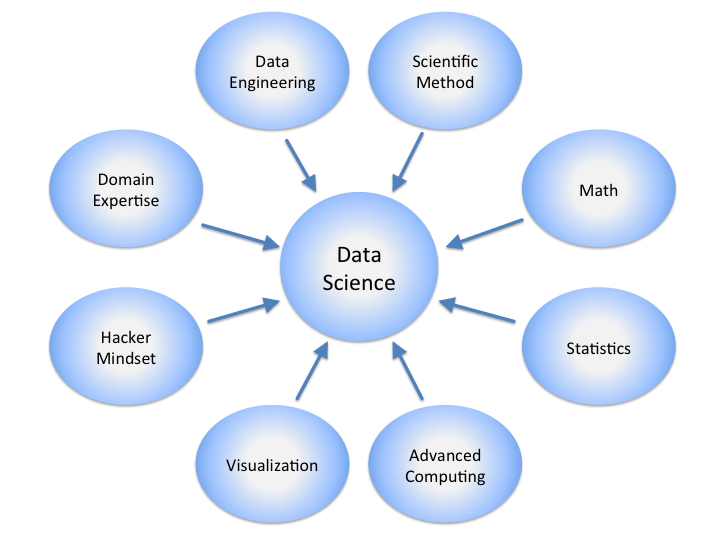
\includegraphics[width=.8\textwidth]{fig/data_science}
    \end{center}
    \footnotesize{forrás: wikipedia.org}
\end{frame}

\begin{frame}{Adatbányászat}
    \begin{quote}
        The nontrivial extraction of implicit, previously
    unknown, and potentially useful information
    from data.
    \end{quote}
    \begin{itemize}
        \item Nem triviális, rejtett
        \item információk és összefüggések feltárása
        \item nagy adathalmazokban.
        \item Ezek felhasználása ismeretlen adatok becslésére.
    \end{itemize}
\end{frame}

\begin{frame}{Mi számít adatbányászatnak?}
    Példa: élelmiszerüzlet
    \begin{itemize}
        \item Vásárlók száma
            \begin{itemize}
                \item triviális információ
            \end{itemize}
        \item Előző havi bevétel
            \begin{itemize}
                \item triviális információ
            \end{itemize}
        \item Leggyakrabban együtt vásárolt termékek
            \begin{itemize}
                \item \emph{gyakori elemhalmazok keresése}
                \item \emph{frequent itemsets}
            \end{itemize}
        \item Hány kasszát kell kinyitni pénteken 16 órakkor?
            \begin{itemize}
                \item vevőszám és vevő kiszolgálási idejének modellezése
                \item \emph{idősorok elemzése}
            \end{itemize}
    \end{itemize}
\end{frame}

\begin{frame}{Multidiszciplináris terület}
    \begin{description}
        \item[matematika] lineáris algebra, mátrixalgebra, optimalizáció, statisztika
        \item[informatika] adatgyűjtés, adattisztítás, gépi tanuló algoritmusok használata
        \item[egyéb] bioinformatika, számítógépes nyelvészet, társadalomtudományok
    \end{description}
\end{frame}

\begin{frame}{Adatok reprezentációja I.}
    \begin{itemize}
        \item Vektor-tér modell
            \begin{itemize}
                \item egy megfigyeléshez egy vektor tartozik
                \item a megfigyelt tér tulajdonságainak(feature-ök) száma adja a vektorok dimenzióját
                \item pl.~spamdetekció esetén egy emailhez egy vektor tartozik
                \item A vektor dimenziója választható
            \end{itemize}
    \end{itemize}
\end{frame}

\begin{frame}{Adatok reprezentációja II.}
    \begin{itemize}
        \item Idősor
            \begin{itemize}
                \item természetes rendezést adó dimenzió szerinti adatok
                \item pl.~napi csapadékmennyiség 2014-ben a 11.~kerületben
            \end{itemize}
        \item Gráf
            \begin{itemize}
                \item egymással valamilyen kapcsolatban álló adatok (pl.~oksági kapcsolat)
                \item pl.~betegségek kialakulásának modellezése
                \item pl.~Über utazások
            \end{itemize}
    \end{itemize}
    A helyes reprezentáció választása kulcsfontosságú.
\end{frame}

\begin{frame}{Adatok vektoros reprezentációja}
    \begin{itemize}
        \item minta (sample): egy elem reprezentációja - \textcolor{darkred}{vektor}
        \item jegy (feature): egyetlen jellemző - \textcolor{darkred}{a vektor egy eleme}. Bármi lehet egy feature, pl. email esetén:
	\begin{itemize}
		\item email hossza
		\item email feladója
		\item tartalmazza-e a ,,Rolex'' szót?
		\item tartalmazza-e a ,,Trust fund'' kifejezést?
	\end{itemize}
		\item címke (label): ,,válasz''

    \end{itemize}
\end{frame}

\begin{frame}{Tanitó, Validációs és Teszthalmaz}
\begin{itemize}
        \item tanítóhalmaz (training dataset): tanításra használt minták - \textcolor{darkred}{mátrix}
		\item validációs halmaz: paraméterek beállítására, illetve a tanítás korai leállítására használt halmaz. Tanitás közben mérhető vele az algoritmus teljesítménye
		\item teszthalmaz: tanítás utáni tesztelésre használt halmaz. Csak egyszer futtatható rajta az algoritmus
	\end{itemize}
\centering
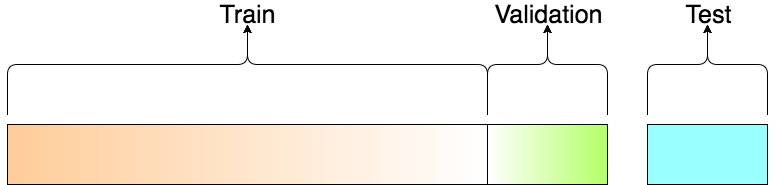
\includegraphics[width=.8\textwidth]{fig/train}
\end{frame}

\begin{frame}{Adatok típusai}
    \begin{enumerate}
        \item címkézett vs.~címkézetlen
            \begin{itemize}
                \item címkézett
                    \begin{itemize}
                        \item tudjuk a jó választ
                        \item pl.~filmek értékelései
                        \item sokszor kevés adatunk van, előállítása drága
                        \item \emph{felügyelt tanulás}
                    \end{itemize}
                \item címkézetlen
                    \begin{itemize}
                        \item nem tudjuk a jó választ
                        \item pl.~internetes kommentek
                        \item ebből általában jóval több van
                        \item \emph{felügyeletlen tanulás}
                    \end{itemize}
            \end{itemize}
        \item folytonos vs.~diszkrét
    \end{enumerate}
\end{frame}

\begin{frame}{Adatbányászat folyamata}
    \begin{enumerate}
        \item Adattisztítás
            \begin{itemize}
                \item Zajszűrés, outlier szűrés
                \item Hiányzó adatok kezelése
            \end{itemize}
        \item Mintavételezés (szükség esetén)
            \begin{itemize}
                \item Ha túl sok az adat 
            \end{itemize}
        \item Adattranszformáció
            \begin{itemize}
                \item Dimenziócsökkentés (egyre kevésbé)
                \item Normalizálás, standardizálás
            \end{itemize}
        \item Adatbányászati algoritmus futtatása
        \item Kiértékelés
    \end{enumerate}
\end{frame}


\begin{frame}{Felügyelt és felügyeletlen tanulás}
\begin{itemize}
	\item A \textbf{felügyelt} tanulás
	\begin{itemize}
		\item Olyan probléma, ahol a bemeneti adathoz(x) tartozik egy kimeneti változó(y)
		\item A kimeneti adatok elkészitése általában emberi erőforrások bevonásával történik - Cimkézett adat		
	\end{itemize}
	\item A \textbf{felügyeletlen} tanulás
	\begin{itemize}
		\item A probléma során csak a bemeneti változó(x) áll rendelkezésünkre
		\item Hasznos, mivel a Cimkézett adat drága
	\end{itemize}
\end{itemize}
\end{frame}

\begin{frame}{Feladattípusok}
    \begin{itemize}
        \item Osztályozás (O) \visible<2->{-- \textcolor{darkred}{felügyelt, diszkrét osztályok}}
            \begin{itemize}
                \item Elemek besorolása előre meghatározott halmazokba
                \item pl.~spam vagy ham egy levél
            \end{itemize}
        \item Regresszió (R) \visible<3->{-- \textcolor{darkred}{felügyelt, folytonos célváltozó}}
            \begin{itemize}
                \item Elemek attribútumai közti kapcsolatok modellezése
                \item pl.~lakásárak előrejelzése méret, elhelyezkedést stb.~alapján
            \end{itemize}
        \item Klaszterezés (K) \visible<4->{-- \textcolor{darkred}{felügyeleletlen, diszkrét klaszterek}}
            \begin{itemize}
                \item Elemek csoportosítása valamilyen hasonlósági metrika szerint
                \item Cél: azonos klaszterben lévő elemek ,,hasonlítsanak'' egymásra, eltérő klaszterben lévők minél kevébé.
                \item pl.~marketszegmentálás
            \end{itemize}
    \end{itemize}
\end{frame}

%\begin{frame}{Gyakori feladatok II.}
%    \begin{itemize}
%        \item Idősorok elemzése
%            \begin{itemize}
%                \item Időhöz kapcsolt megfigyelések alapján előrejelzések, minták keresése
 %           \end{itemize}
 %       \item Gyakori halmazok keresése
 %           \begin{itemize}
 %               \item pl.~Milyen termékeket vásárolnak gyakran együtt az emberek?
 %           \end{itemize}
  %      \item Ajánlórendszerek
   % \end{itemize}
%\end{frame}

\begin{frame}{Tipikus algoritmusok}
\begin{itemize}
	\item Support vector machine (Osztályozás, Regresszió)
	\item Decision Tree (Osztályozás, Regresszió)
	\item Random Forest (Osztályozás, Regresszió)
	\item Logistic Regression (Osztályozás)
	\item Linear Regression (Regresszió)
	\item Neural Networks (Osztályozás, Regresszió)
	\item K-means (Klaszterezés)
	\item LDA (Klaszterezés)

\end{itemize}

\footnotesize{Tovább olvasható: https://scikit-learn.org/stable/}
\end{frame}

\begin{frame}{Kiértékelés}
    \begin{itemize}
        \item Osztályozás
            \begin{itemize}
                \item confusion matrix alapján:
                \item pontosság (precision), fedés (recall), F-mérték (F-score)
            \end{itemize}
        \item Regresszió
            \begin{itemize}
                \item átlagos négyzetes hiba (RMSE), abszolút hiba
            \end{itemize}
        \item Klaszterezés
            \begin{itemize}
                \item nagyon nehéz kiértékelni
                \item klaszterek minősége (mennyire tömör, milyen távol vannak egymástól)
            \end{itemize}
    \end{itemize}
\end{frame}

\begin{frame}{Bináris osztályozás kiértékelése}

    \begin{center}
\includegraphics[width=.8\textwidth]{true_pos}
    \end{center}

\end{frame}

\begin{frame}{Bináris osztályozás kiértékelése}

Precision: milyen arányban helyesek a pozitív válaszaink.
\begin{equation*}
	\text{Precision}=\frac{tp}{tp+fp}
\end{equation*}

Recall: mennyit találtunk meg az összes pozitív címkéjű elemből.
\begin{equation*}
	\text{Recall}=\frac{tp}{tp+fn}
\end{equation*}

\end{frame}

\begin{frame}{Kiértékelés - F-score}
    \begin{itemize}
            \item a kettő között tradeoff van
                \item F-score
    \end{itemize}

    \begin{equation*}
        \text{F-score} = 2 * \frac{\text{prec}  \text{rec}}{\text{prec} + \text{rec}}
    \end{equation*}
\end{frame}
\begin{frame}{Technológiai háttér}
    \begin{itemize}
        \item Python, Java, R statisztikai csomag, Lua
        \item Linux
        \item gépi tanulás: scikit-learn (Python), Weka (Java)
        \item deep learning: TensorFlow, PyTorch, Keras stb.
        \item plain text, CSV, TSV, esetleg XML
    \end{itemize}
\end{frame}

\begin{frame}{Deep learning}
    \begin{itemize}
    	\item eddig tradicionális Machine Learning-ről beszéltünk
        \item feladatspecifikus modellek helyett a reprezentációt tanulja
        \item biológiai interpretáció
        \item miért tértek vissza?
            \begin{itemize}
                \item egyre gyorsabb GPU-k
                \item ügyes inicializációs módszerek
                \item ügyes architektúrák
            \end{itemize}
    \end{itemize}
\end{frame}

\begin{frame}{ML vs Deep Learning}
	\centering
	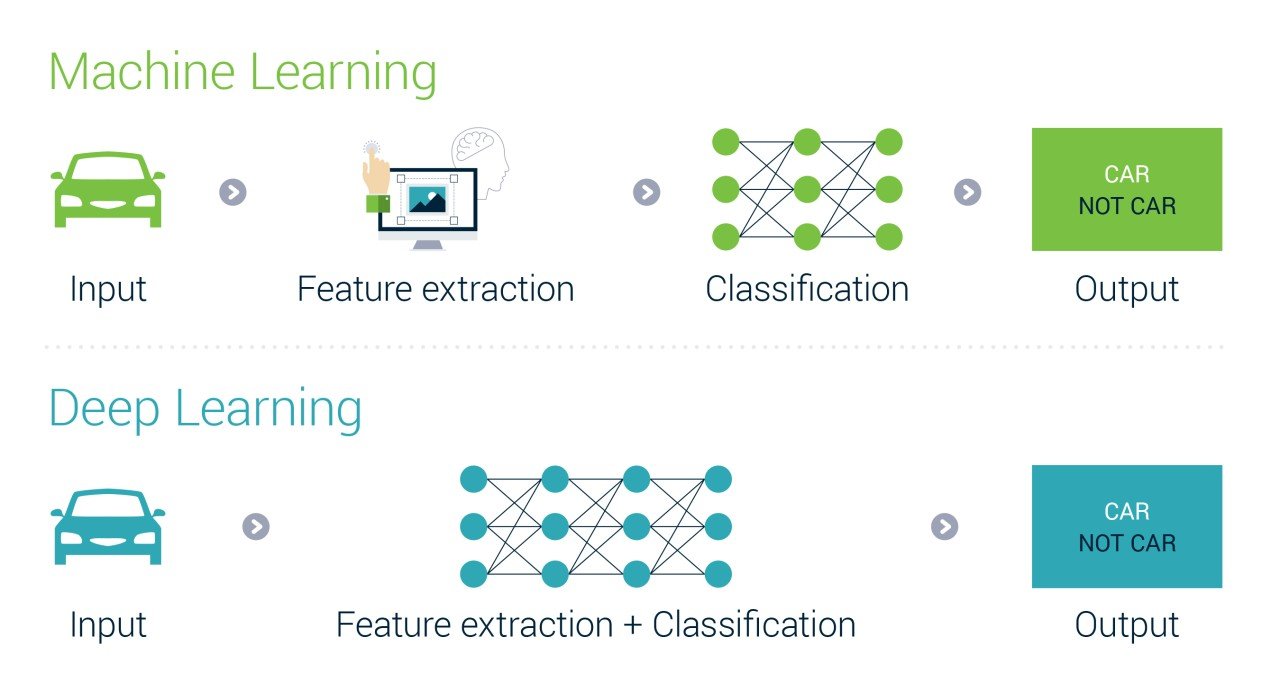
\includegraphics[width=.8\textwidth]{fig/ml}
\end{frame}

\begin{frame}{ML vs Deep Learning}
\begin{itemize}
	\item Deep learning
	\begin{itemize}
		\item Automatikus feature kiválasztás
		\item Nagy adattal jól skálázódik
		\item Képes nem lineárisan szeparálható problémák megoldására is
		\item Jelenleg a legjobb eredményeket elérő technikák
	\end{itemize}
\item Klasszikus Machine Learning
\begin{itemize}
	\item A feature extraction ránk van bizva
	\item Kis adatból is jól tanul
	\item Nagy adattal rosszabban skálázódik mint a DL
	\item Kisebb feladatok esetén "elég" lehet
\end{itemize}
\end{itemize}
\end{frame}

\begin{frame}{Előrecsatolt neurális háló}
    \def\layersep{2.1cm}

\begin{tikzpicture}[shorten >=1pt,->,draw=black!50, node distance=\layersep]
    \tikzstyle{every pin edge}=[<-,shorten <=1pt]
    \tikzstyle{neuron}=[circle,fill=black!25,minimum size=17pt,inner sep=0pt]
    \tikzstyle{input neuron}=[neuron, fill=green!50];
    \tikzstyle{output neuron}=[neuron, fill=red!50];
    \tikzstyle{hidden neuron}=[neuron, fill=blue!50];
    \tikzstyle{annot} = [text width=3em, text centered]

    % Draw the input layer nodes
    \foreach \name / \y in {1,...,4}
    % This is the same as writing \foreach \name / \y in {1/1,2/2,3/3,4/4}
        \node[input neuron, pin=left:Input \#\y] (I-\name) at (0,-\y) {};

    % Draw the hidden layer nodes
    \foreach \name / \y in {1,...,5}
        \path[yshift=0.5cm]
            node[hidden neuron] (H-\name) at (\layersep,-\y cm) {};

    \foreach \name / \y in {15,25,35,45}
        \path[yshift=0.5cm]
            node[hidden neuron] (H-\name) at (\layersep+\layersep,-\y mm) {};

    % Draw the output layer node
            \node[output neuron,pin={[pin edge={->}]right:Output}] (O) at (3*\layersep, -25 mm) {};

    % Connect every node in the input layer with every node in the
    % hidden layer.
    \foreach \source in {1,...,4}
        \foreach \dest in {1,...,5}
            \path (I-\source) edge (H-\dest);

    % Connect every node in the hidden layer with the output layer
    \foreach \source in {1,...,5}
        \foreach \dest in {15,25,35,45}
            \path (H-\source) edge (H-\dest);

    \foreach \source in {15,25,35,45}
        \path (H-\source) edge (O);

    % Annotate the layers
    \node[annot,above of=H-1, node distance=1cm] (hl) {Hidden layer 1};
    \node[annot,right of=hl, node distance=\layersep] (hl2) {Hidden layer 2};
    \node[annot,left of=hl] {Input layer};
    \node[annot,right of=hl2] {Output layer};
\end{tikzpicture}
\end{frame}

\begin{frame}{Előrecsatolt neurális háló}
    \begin{equation*}
        \mathbf{h_1} = \sigma (\mathbf{W_1 x})
    \end{equation*}
    \begin{equation*}
        \mathbf{h_2} = \sigma (\mathbf{W_2 h_1})
    \end{equation*}
    \begin{equation*}
        \mathbf{y} = \sigma (\mathbf{W_3 h_2})
    \end{equation*}

$\sigma$ az aktivációs függvény, tipikusan nemlineáris, pl. sigmoid:
    \begin{equation*}
        \sigma(x) = \frac{1}{1 + e^{-x}}
    \end{equation*}

\end{frame}

\begin{frame}{Előrecsatolt neurális háló}
    \begin{itemize}
        \item a bemenet ($\mathbf{x}$) és a kimenet ($y$) adott
        \item a súlyokat tanuljuk (backpropagation)
        \item ez a hálózat kapacitása vagy memóriája
    \end{itemize}
    Hátrányok:
    \begin{itemize}
        \item csak egy irányba folyik az adat (nincs sorrendiség)
        \item hajlamos túltanulni
    \end{itemize}
\end{frame}

\begin{frame}{Rekurrens háló}
    \begin{itemize}
        \item olyan háló, amiben van irányított kör
        \item képes temporális összefüggéseket megtanulni
        \item mintha több előracsatolt hálót kötnénk össze
        \item nyelvfeldolgozásban élenjáró technológia
        \item Long-short term memory (LSTM)
            \begin{itemize}
                \item \emph{memóriával} rendelkező cella, amely képes megjegyezni, illetve elfelejteni korábbi információt
                \item általában több száz cellát tartalmaz egy háló
            \end{itemize}
    \end{itemize}
\end{frame}

\begin{frame}{Rekurrens háló}
	\centering
	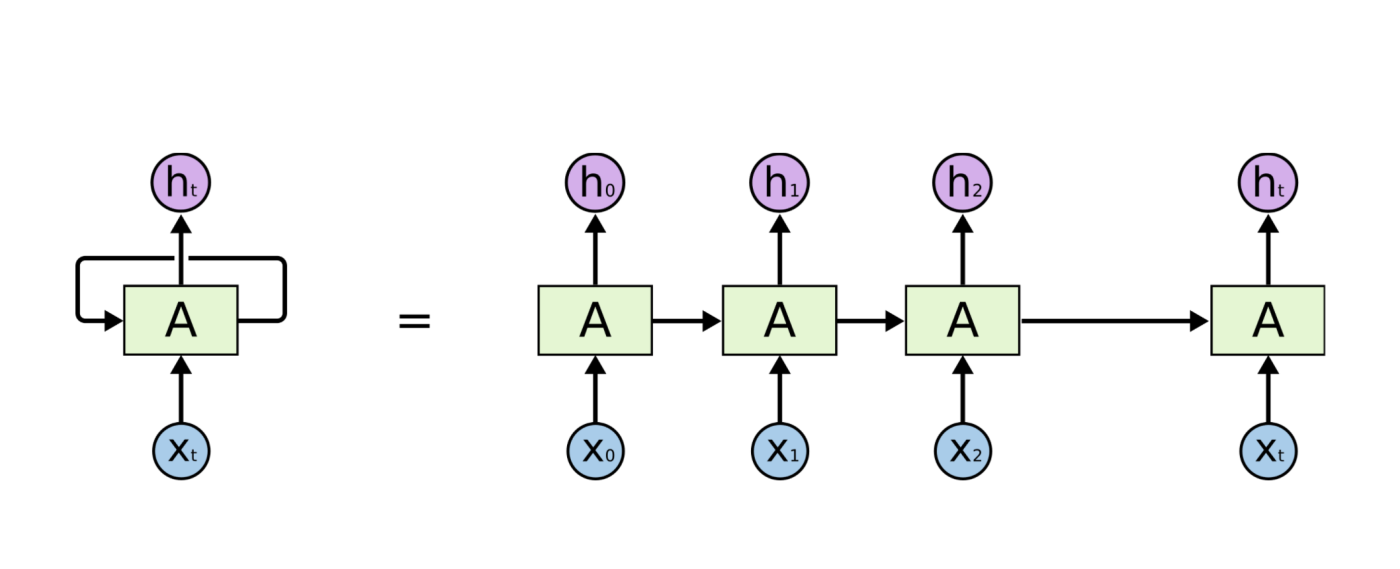
\includegraphics[width=.99\textwidth]{fig/rnn}
\end{frame}

\begin{frame}{Konvolúciós háló}
    \begin{itemize}
        \item térbeli struktúrát figyelembe vevő hálózat - képfeldolgozás
        \item 1D konvolúció szövegre és idősorokra is elterjedt
        \item fontosságot rendel a kép egyes részeihez
        \item ezáltal jobb eredményt ad, mintha csak egy előrecsatolt struktúrába vezetnénk be a kép elemeit
    \end{itemize}
\end{frame}

\begin{frame}{Konvolúciós háló}
\centering
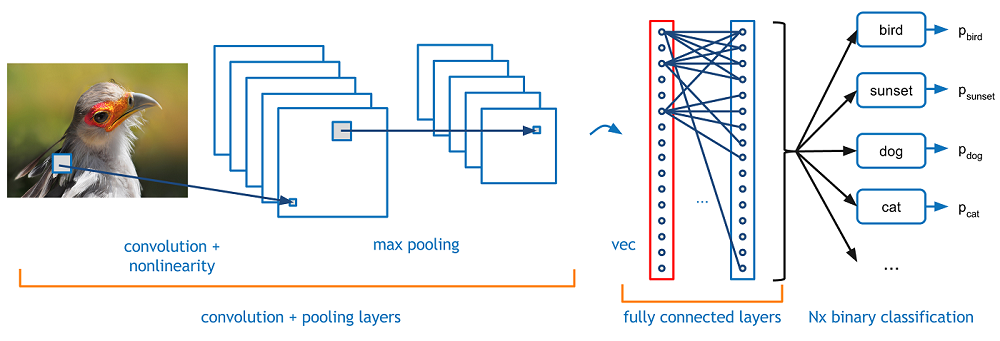
\includegraphics[width=.99\textwidth]{fig/cnn}
\end{frame}

\begin{frame}{További architektúrák}
    \begin{itemize}
        \item Generative adversarial network (GAN)
            \begin{itemize}
                \item két hálózat versenyzik egymással: generátor és diszkriminátor
                \item generátor: próbál valósághű hamisítványokat gyártani
                \item diszkriminátor: próbálja megkülönböztetni a valós adatokat a generátor által hamisítottól
            \end{itemize}
        \item (Variational) autoencoder (VAE)
            \begin{itemize}
                \item a bemenet és a kimenet megegyezik, a háló dolga rekonstruálni a bemenetet
                \item tipikusan jóval kisebb a rejtett rétegben lévő neuronok száma
            \end{itemize}
    \end{itemize}
\end{frame}

\begin{frame}{Adatelemzés}
    \begin{itemize}
        \item adatbányászat- -
        \item mintákat, trendeket keresünk
        \item általában nem cél jósolni
        \item Pandas adatelemző könyvtár - labor tavasszal
    \end{itemize}
\end{frame}

\begin{frame}{Köszönöm a figyelmet.}



\end{frame}
\end{document}
